\chapter{IF and ELSE Statements}\label{CHAP_IfAndElse}

\section{Difficulty: EASY}

\subsubsection*{Exercise 6.E01}
Write a code that accepts an arbitrary number and determines whether the number is
\begin{enumerate}[label=(\alph*)]
	\item positive (larger than zero)
	\item negative (smaller than zero)
	\item neither negative nor positive (zero)
\end{enumerate}
Make sure the code displays your findings to the user.\\


\textit{Hints:
You will need an {\code{IF-ELIF-ELSE}} chain structure for this exercise. The {\code{IF}} case could check whether the number is smaller than zero. The {\code{ELIF}} case could check whether the number is larger than 0 and the {\code{ELSE}} case handles numbers which are equal to zero.}\\[1cm]


% ------------------------------------------------------------------------------


\subsubsection*{Exercise 6.E02}
Write a code that asks the user to enter one letter and then checks whether the letter is a
vowel. The following letters are vowels: a, e, i, o, and u.\\


\textit{Hints:
You can either use an {\code{IF-ELIF-ELSE}} chain statements to check whether the letter the user has entered is equal to any of the vowels or you could use a simple {\code{IF-ELSE}} statement with a more complex conditional test (using the {\code{OR}} operator).}\\[1cm]


% ------------------------------------------------------------------------------

\newpage
\subsubsection*{Exercise 6.E03 \red{[M]}}
Write a code that accepts an arbitrary number and determines whether the number is
\begin{enumerate}[label=(\alph*)]
	\item even
	\item odd
\end{enumerate}


\textit{Hints:
To determine whether a number is even or odd calculate the remainder of a division by two.The remainder of an even number divided by two is always zero. The remainder of an odd
number divided by two is always 1. The remainder can be calculated using the modulus
operator \%.}\\[1cm]


% ------------------------------------------------------------------------------

\subsubsection*{Exercise 6.E04}
Write a code that asks the user to enter their name and their nationality (eng, fr, de, esp, it, etc.). Then greet the user with a personalised message based on their first language:\\
\hspace*{5mm}English (eng): {\code{"Good morning, [NAME]!"}}\\
\hspace*{5mm}French (fr): {\code{"Bonjour, [NAME]!"}}\\
\hspace*{5mm}German (de): {\code{"Guten Morgen, [NAME]!"}}\\
\hspace*{5mm}Spanish (esp): {\code{"Buenos dias, [NAME]!"}}\\
\hspace*{5mm}Italien (it): {\code{"Buongiorno, [NAME]!"}}\\
where {\code{[NAME]}} is a place holder for the name the user has entered. Add more greetings in different languages if you know more! :)\\


\textit{Hints:
Use an {\code{IF-ELIF-ELSE}} chain statement to check the nationality against the available
options. Remember to use the {\code{==}} operator to check whether two strings are the same.}\\[1cm]


% ------------------------------------------------------------------------------

\subsubsection*{Exercise 6.E05}
Write a code that acts as a virtual bouncer. The virtual bouncer should ask the user how old
they are. If the user is 18 or older they are allowed to come in. If they are younger than 18,
the virtual bouncer will ask them to leave.\\


\textit{Hints:
When you accept user input the input will always be of primitive data type {\code{string}}. If you want to perform mathematical operations on the input you need to convert it into a number
first. This can be done with the {\code{int()}} function.}


% ------------------------------------------------------------------------------

\newpage
\section{Difficulty: MEDIUM}


\subsubsection*{Exercise 6.M01}
Write code that acts like a virtual ATM machine. At the beginning specify an account
balance. Then allow the user to withdraw money. The ATM does not allow any overdrafts. If
enough money is in the account, the ATM will carry out the transaction and display the new
account balance. If not enough money is in the account the ATM will refuse to carry out the
transaction.\\


\textit{Hints:
Remember you will need to convert the input from string type to float type using the
{\code{float()}} function. Check whether the account balance would be negative after the transaction. If so, the code should not allow the transaction.}\\[1cm]


% ------------------------------------------------------------------------------

\subsubsection*{Exercise 6.M02}
Write a code that asks the user for the day of the week and the time (in full hours and 24h
format) and determines whether a shop is currently open. The shopping hours are:\\
\hspace*{5mm}Monday to Saturday: 7am to 10pm\\
\hspace*{5mm}Sunday: 10am to 5pm\\


\textit{Hints:
Remember you will need to convert the input from string type to integer type using the
{\code{int()}} function. Using a nested IF-ELSE statement will reduce the amount of code you will have to write.}\\[1cm]


% ------------------------------------------------------------------------------

\subsubsection*{Exercise 6.M03 \red{[M]}}
A year $y$ is a leap year if it is exactly divisible by four unless it’s also exactly divisible by 100 and at the same time not exactly divisible by 400.\\
Ask the user for a year and then determine whether it is a leap year or not.\\


\textit{Hints:
Remember you will need to convert input from string type to integer type using the {\code{int()}} function before performing mathematical operations. To check whether a number is exactly divisible by another number check whether the modulus \% is zero.}\\[1cm]


% ------------------------------------------------------------------------------

\subsubsection*{Exercise 6.M04}
Write a code that asks the user for a month and a day and returns the season.
The seasons are determined as follows:\\
\hspace*{5mm}Spring: 21st of March to 20th of June\\
\hspace*{5mm}Summer: 21st of June to 20th of September\\
\hspace*{5mm}Autumn: 21st of September to 20th of December\\
\hspace*{5mm}Winter: 21st of December to 20th of March\\


\textit{Hints:
Remember you will need to convert input from string type to integer type using the {\code{int()}} function before performing mathematical operations.}
\\[1cm]


% ------------------------------------------------------------------------------

\subsubsection*{Exercise 6.M05}
Write a code that asks the user to enter a string. Then determine whether the string is a
palindrome. A palindrome is a word which reads the same forward or backwards. For example: "Anna" or "Madam".\\


\textit{Hints:
If you want to reverse string {\code{str}} type {\code{str[::-1]}}. This will generate a substring from the original string from the beginning to the end with step -1. Meaning the string will be built from the end towards the beginning. Play around with the string reverse operation a bit before tackling the exercise. You might also find the {\code{lower()}} function useful when comparing the strings.}\\[1cm]


% ------------------------------------------------------------------------------

\subsubsection*{Exercise 6.M06}
Write a code that accepts three numbers and
\begin{enumerate}[label=(\alph*)]
	\item returns the maximum
	\item returns the minimum
\end{enumerate}


\textit{Hints:
Use a nested {\code{IF-ELSE}} statement. Pick two numbers first and check which one is larger. Then compare this number to the third number to determine the overall largest number. Do the
same for the minimum.}


% ------------------------------------------------------------------------------

\newpage
\section{Difficulty: HARD}

\subsubsection*{Exercise 6.H01}
An Armstrong number (also known as narcissistic number) is a number that is the sum of its
own digits each raised to the power of the digit number.\\
For example: $153 \rightarrow 1^3 + 5^3 + 3^3 = 1 + 125 + 27 = 153$\\
Write a code that asks the user to provide a three-digit integer. Then check whether the
number is an Armstrong number. Display your result.\\


Hints:
The four three-digit Armstrong numbers are: 153, 370, 371, 407.
You will need to convert string characters into numbers using the {\code{int()}} function. To extract individual characters from a string use the corresponding string indices.\\[1cm]


% ------------------------------------------------------------------------------

\subsubsection*{Exercise 6.H02}
Consider the following chess board layout:
\begin{figure}[H]
		\centering
		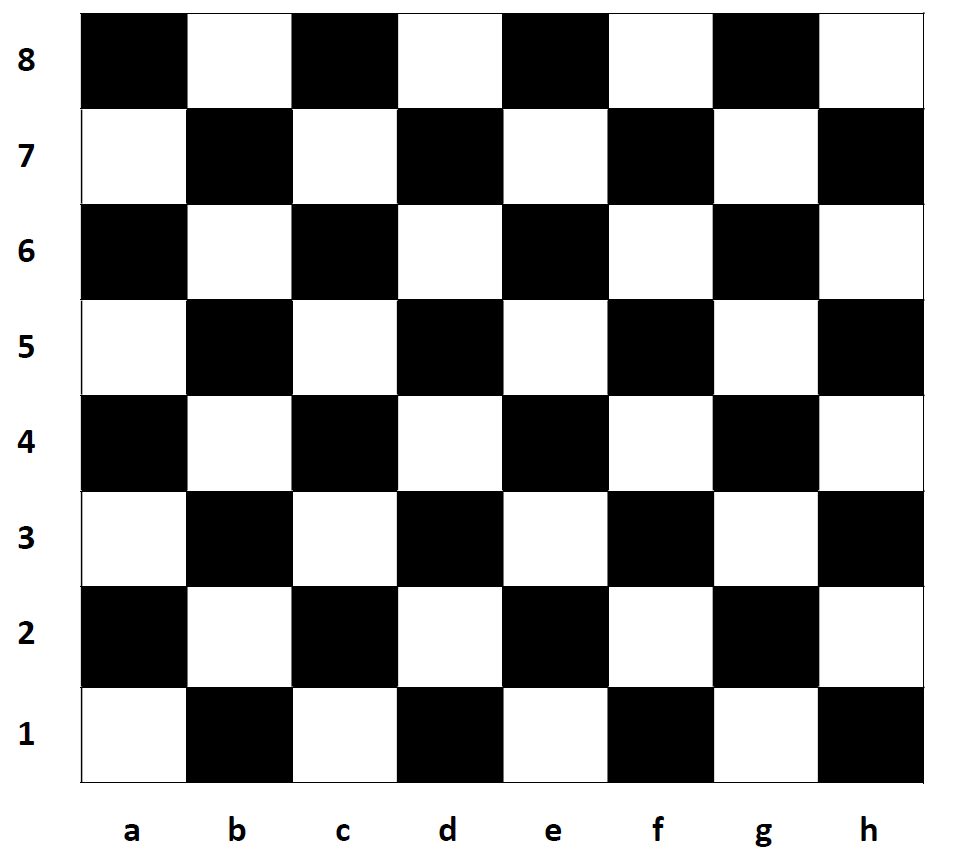
\includegraphics[width=0.7\textwidth]{../IMG/6H02.png} 
\end{figure}

Every square on the board is identified by a number and a letter (for example: The lower left
corner is identified by \textbf{1a}).\\
Write a code that asks the user for a square identifier and then determines whether the
square in question is white or black.\\


\textit{Hints:
Try to find a pattern before you start writing a code. Which conditions need to be met by the
number part of the ID and which conditions need to be met by the letter part of the ID for the
square to be either black or white?\\
Remember: You can check whether a number is even or odd by calculating the modulus \%.
The modulus 2 of an even number is zero, the modulus 2 of an odd number is 1.}

